\subsection{Ambito utente}

\hypertarget{U0}{}
\bookmark[dest=U0,level=3]{UCU 0: Caso base utente generico}
\subsubsection{UCU 0: Caso base utente generico}
\begin{figure}[H]
\centering
\includegraphics[trim=0cm 0.8cm 0cm 0cm,clip=true,scale=0.75]%
{./grafici/U0}
\caption{UCU 0: Caso base utente generico}
\end{figure}
\begin{itemize}
\item \textbf{Attori:} Utente;
\item \textbf{Descrizione:} L'utente accede alla pagina principale e, per poter accedere alle principali funzionalità, deve autenticarsi.
L'utente non autenticato può registrarsi oppure effettuare il \textit{login} se è già registrato diventando utente autenticato.
\item \textbf{Precondizione:} Il sistema è operativo e l'utente ha iniziato ad interfacciarvisi;
\item \textbf{Scenario principale:}
\begin{itemize}
\item L'utente può effettuare la registrazione (UCU 1);
\item L'utente può effettuare il \textit{login} e diventare autenticato (UCU 2);
\end{itemize}
%\item \textbf{Scenario alternativo:}
%\item \textbf{Inclusioni:}
\item \textbf{Postcondizione:} Il sistema ha eseguito le operazioni desiderate dall'utente.
\end{itemize}

\hypertarget{U1}{}
\bookmark[dest=U1,level=4]{UCU 1: Registrazione}
\subsubsection{UCU 1: Registrazione}
\begin{figure}[H]
\centering
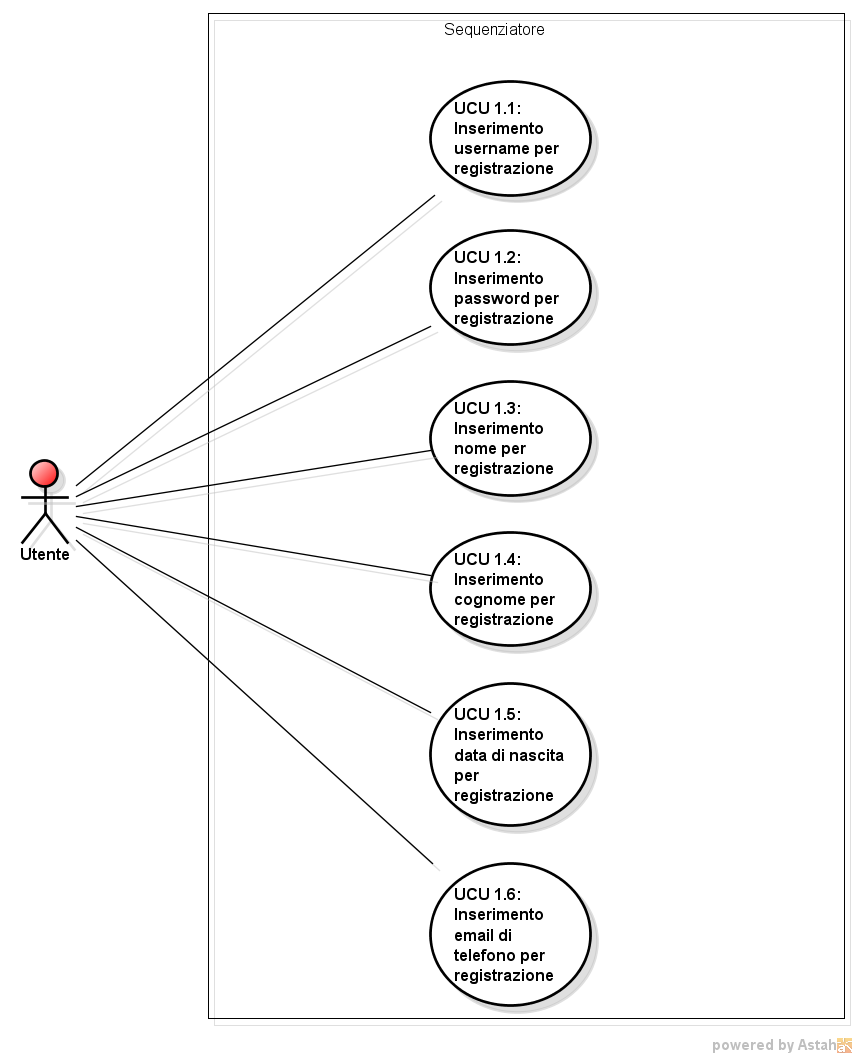
\includegraphics[trim=0cm 0.8cm 0cm 0cm,clip=true,width=%
\textwidth]
{./grafici/U1}
\caption{UCU 1: Registrazione}
\end{figure}
\begin{itemize}
	\item \textbf{Attori:} Utente;
	\item \textbf{Descrizione:} L'utente può registrarsi inserendo i dati richiesti dal sistema;
	\item \textbf{Precondizione:} Il sistema é operativo e l'utente ha richiesto la registrazione;
	\item \textbf{Scenario principale:}
	\begin{itemize}
		\item L'utente inserisce lo \textit{username} scelto (UCU 1.1);
		\item L'utente inserisce la \textit{password} scelta (UCU 1.2);
		\item L'utente inserisce il proprio nome (UCU 1.3);
		\item L'utente inserisce il proprio cognome (UCU 1.4);
		\item L'utente inserisce la propria data di nascita (UCU 1.5);
		%\item L'utente inserisce un proprio numero di telefono.
		\item L'utente inserisce la propria \textit{email} (UCU 1.6).
	\end{itemize}
	\item \textbf{Scenario alternativo:}
	\begin{itemize}
		\item Un altro utente possiede lo stesso \textit{username} scelto dall'utente che viene avvisato dell'errore e può scegliere un \textit{username} diverso;
	\end{itemize}
	\item \textbf{Postcondizione:} Il sistema ha salvato i dati immessi dall'utente che ora può autenticarsi.
\end{itemize}

\hypertarget{U1.1}{}
\bookmark[dest=U1.1,level=5]{UCU 1.1: Inserimento username per registrazione}
\subsubsection{UCU 1.1: Inserimento username per registrazione}
\begin{itemize}
	\item \textbf{Attori:} Utente;
	\item \textbf{Descrizione:} L'utente può inserire il proprio \textit{username};
	\item \textbf{Precondizione:} L'utente ha richiesto la registrazione e vuole inserire lo \textit{username} scelto;
	\item \textbf{Scenario principale:} L'utente inserisce il proprio \textit{username};
	\item \textbf{Postcondizione:} Lo \textit{username} è stato inserito e il sistema prosegue con la registrazione.
\end{itemize}

\hypertarget{U1.2}{}
\bookmark[dest=U1.2,level=5]{UCU 1.2: Inserimento password per registrazione}
\subsubsection{UCU 1.2: Inserimento password per registrazione}
\begin{itemize}
	\item \textbf{Attori:} Utente;
	\item \textbf{Descrizione:} L'utente può inserire la propria \textit{password};
	\item \textbf{Precondizione:} L'utente ha richiesto la registrazione e vuole inserire la \textit{password} scelta;
	\item \textbf{Scenario principale:} L'utente può inserire la propria \textit{password};
	\item \textbf{Postcondizione:} La \textit{password} è stata inserita e il sistema prosegue con la registrazione.
\end{itemize}

\hypertarget{U1.3}{}
\bookmark[dest=U1.3,level=5]{UCU 1.3: Inserimento nome per registrazione}
\subsubsection{UCU 1.3: Inserimento nome per registrazione}
\begin{itemize}
	\item \textbf{Attori:} Utente;
	\item \textbf{Descrizione:} L'utente può inserire il proprio nome;
	\item \textbf{Precondizione:} L'utente ha richiesto la registrazione e vuole inserire il proprio nome;
	\item \textbf{Scenario principale:} L'utente può inserire il proprio nome;
	\item \textbf{Postcondizione:} Il nome è stato inserito e il sistema prosegue con la registrazione.
\end{itemize}

\hypertarget{U1.4}{}
\bookmark[dest=U1.4,level=5]{UCU 1.4: Inserimento cognome per registrazione}
\subsubsection{UCU 1.4: Inserimento cognome per registrazione}
\begin{itemize}
	\item \textbf{Attori:} Utente;
	\item \textbf{Descrizione:} L'utente può inserire il proprio cognome;
	\item \textbf{Precondizione:} L'utente ha richiesto la registrazione e vuole inserire il proprio cognome;
	\item \textbf{Scenario principale:} L'utente può inserire il proprio cognome;
	\item \textbf{Postcondizione:} Il cognome è stato inserito e il sistema prosegue con la registrazione.
\end{itemize}

\hypertarget{U1.5}{}
\bookmark[dest=U1.5,level=5]{UCU 1.5: Inserimento data di nascita per registrazione}
\subsubsection{UCU 1.5: Inserimento data di nascita per registrazione}
\begin{itemize}
	\item \textbf{Attori:} Utente;
	\item \textbf{Descrizione:} L'utente può inserire la propria data di nascita;
	\item \textbf{Precondizione:} L'utente ha richiesto la registrazione e vuole inserire la propria data di nascita;
	\item \textbf{Scenario principale:} L'utente può inserire la propria data di nascita;
	\item \textbf{Postcondizione:} La data di nascita è stata inserita e il sistema prosegue con la registrazione.
\end{itemize}

\hypertarget{U1.6}{}
\bookmark[dest=U1.6,level=5]{UCU 1.6: Inserimento email per registrazione}
\subsubsection{UCU 1.6: Inserimento email per registrazione}
\begin{itemize}
	\item \textbf{Attori:} Utente;
	\item \textbf{Descrizione:} L'utente può inserire una sua \textit{email};
	\item \textbf{Precondizione:} L'utente ha richiesto la registrazione e vuole inserire la propria \textit{email};
	\item \textbf{Scenario principale:} L'utente può inserire una sua \textit{email};
\item \textbf{Postcondizione:} L'\textit{email} è stata inserita e il sistema prosegue con la registrazione utente.
\end{itemize}

\hypertarget{U2}{}
\bookmark[dest=U2,level=4]{UCU 2: Login}
\subsubsection{UCU 2: Login}
\begin{figure}[H]
\centering
\includegraphics[trim=0cm 0.8cm 0cm 0cm,clip=true,scale=0.75]%
{./grafici/U2}
\caption{UCU 2: Login}
\end{figure}
\begin{itemize}
\item \textbf{Attori:} Utente;
\item \textbf{Descrizione:} L'utente può inserire i propri dati d'accesso, ossia lo \textit{username} e la propria \textit{password}. Se lo \textit{username} appartiene all'insieme degli utenti del sistema e la relativa \textit{password} è corretta, allora l'utente viene autenticato;
\item \textbf{Precondizione:} Il sistema è operativo e l'utente non autenticato vuole effettuare il \textit{login};
\item \textbf{Scenario principale:}
\begin{itemize}
\item L'utente inserisce il proprio \textit{username} (UCU 2.1);
\item L'utente inserisce la propria \textit{password} (UCU 2.2).
\end{itemize}
\item \textbf{Scenario alternativo:}
\begin{itemize}
\item Le credenziali non risultano essere corrette, viene dunque segnalato l'errore all'utente che può reinserire i dati.
\end{itemize}
\item \textbf{Postcondizione:} L'utente diventa autenticato e il sistema è pronto per consentire la gestione dei processi.
\end{itemize}

\hypertarget{U2.1}{}
\bookmark[dest=U2.1,level=5]{UCU 2.1: Inserimento username per login}
\subsubsection{UCU 2.1: Inserimento username per login}
\begin{itemize}
\item \textbf{Attori:} Utente;
\item \textbf{Descrizione:} L'utente può inserire il proprio \textit{username};
\item \textbf{Precondizione:} L'utente ha richiesto il \textit{login} e vuole inserire la propria data di nascita;
\item \textbf{Scenario principale:} L'utente può inserire il proprio \textit{username};
\item \textbf{Postcondizione:} Lo \textit{username} è stato inserito e il sistema prosegue con la procedura di autenticazione utente.
\end{itemize}

\hypertarget{U2.2}{}
\bookmark[dest=U2.2,level=5]{UCU 2.2: Inserimento password per login}
\subsubsection{UCU 2.2: Inserimento password per login}
\begin{itemize}
\item \textbf{Attori:} Utente;
\item \textbf{Descrizione:} L'utente può inserire la propria \textit{password};
\item \textbf{Precondizione:} L'utente ha richiesto il \textit{login} e vuole inserire la propria \textit{password};
\item \textbf{Scenario principale:} L'utente può inserire la propria \textit{password};
\item \textbf{Postcondizione:} La \textit{password} è stata inserita e il sistema prosegue con la procedura di autenticazione utente.
\end{itemize}

\hypertarget{L0}{}
\bookmark[dest=L0,level=3]{UCL 0: Caso base utente autenticato}
\subsubsection{UCL 0: Caso base utente autenticato}
\begin{figure}[H]
\centering
\includegraphics[trim=0cm 0.8cm 0cm 0cm,clip=true,scale=0.75]%
{./grafici/L0}
\caption{UCL 0: Caso base utente autenticato}
\end{figure}
\begin{itemize}
\item \textbf{Attori:} Utente autenticato;
\item \textbf{Descrizione:} L'utente accede alla pagina principale e, per poter accedere alle principali funzionalità, deve autenticarsi.
L'utente autenticato può gestire il proprio account, gestire un insieme di processi ed effettuare il \textit{logout}, ritornando allo stato di utente non autenticato;
\item \textbf{Precondizione:} Il sistema è operativo, l'utente autenticato ha iniziato ad interfacciarvisi;
\item \textbf{Scenario principale:}
\begin{itemize}
\item L'utente autenticato può gestire il proprio account (UCL 1);
\item L'utente autenticato può gestire i processi disponibili (UCL 2);
\item L'utente autenticato può effettuare il \textit{logout} diventando utente generico (UCL 3).
\end{itemize}
%\item \textbf{Scenario alternativo:}
%\item \textbf{Inclusioni:}
\item \textbf{Postcondizione:} Il sistema ha eseguito le operazioni desiderate dall'utente, salvando eventuali modifiche effettuate all'account e ai processi gestiti.
\end{itemize}

\hypertarget{L1}{}
\bookmark[dest=L1,level=4]{UCL 1: Gestione dell'account}
\subsubsection{UCL 1: Gestione dell'account} %opt
\begin{figure}[H]
\centering
\includegraphics[trim=0cm 0.8cm 0cm 0cm,clip=true,scale=0.75]%
{./grafici/L1}
\caption{UCL 1: Gestione dell'account}
\end{figure}
\begin{itemize}
	\item \textbf{Attori:} Utente autenticato;
	\item \textbf{Descrizione:} L'utente visualizza i dati salvati nel sistema relativi al suo account e può modificarli;
	\item \textbf{Precondizione:} L'utente autenticato vuole gestire i propri dati;
	\item \textbf{Scenario principale:}
	\begin{itemize}
		\item L'utente può visualizzare i propri dati (UCL 1.1);
		\item L'utente può modificare i propri dati (UCL 1.2).
	\end{itemize}
	\item \textbf{Postcondizione:} Il sistema ha eseguito e salvato le operazioni effettuate dall'utente sui dati del suo account.
\end{itemize}

\hypertarget{L1.1}{}
\bookmark[dest=L1.1,level=5]{UCL 1.1: Visualizzazione dei dati dell'utente}
\subsubsection{UCL 1.1: Visualizzazione dei dati dell'utente}
\begin{figure}[H]
\centering
\includegraphics[trim=0cm 0.8cm 0cm 0cm,clip=true,scale=0.75]%
{./grafici/L11}
\caption{UCL 1.1: Visualizzazione dei dati dell'utente}
\end{figure}
\begin{itemize}
	\item \textbf{Attori:} Utente autenticato;
	\item \textbf{Descrizione:} L'utente può visualizzare i dati salvati nel sistema relativi al suo account;
	\item \textbf{Precondizione:} L'utente vuole gestire i suoi dati;
	\item \textbf{Scenario principale:}
	\begin{itemize}
		\item L'utente visualizza il suo \textit{username} (UCL 1.1.1);
		\item L'utente visualizza il suo nome (UCL 1.1.2);
		\item L'utente visualizza il suo cognome (UCL 1.1.3);
		\item L'utente visualizza la sua data di nascita (UCL 1.1.4);
		\item L'utente visualizza la sua \textit{email} (UCL 1.1.5).
		%\item L'utente visualizza il suo numero di telefono.
	\end{itemize}
	\item \textbf{Postcondizione:} Il sistema ha visualizzato i dati dell'account dell'utente.
\end{itemize}

\hypertarget{L1.1.1}{}
\bookmark[dest=L1.1.1,level=5]{UCL 1.1.1: Visualizzazione username}
\subsubsection{UCL 1.1.1: Visualizzazione username}
\begin{itemize}
	\item \textbf{Attori:} Utente autenticato;
	\item \textbf{Descrizione:} L'utente può visualizzare il suo \textit{username};
	\item \textbf{Precondizione:} L'utente vuole visualizzare i suoi dati;
	\item \textbf{Scenario principale:} L'utente può visualizzare il suo \textit{username};
\item \textbf{Postcondizione:} Il sistema ha visualizzato lo \textit{username} dell'utente.
\end{itemize}

\hypertarget{L1.1.2}{}
\bookmark[dest=L1.1.2,level=5]{UCL 1.1.2: Visualizzazione nome}
\subsubsection{UCL 1.1.2: Visualizzazione nome}
\begin{itemize}
	\item \textbf{Attori:} Utente autenticato;
	\item \textbf{Descrizione:} L'utente può visualizzare il suo nome;
	\item \textbf{Precondizione:} L'utente vuole visualizzare i suoi dati;\\
	\item \textbf{Scenario principale:} L'utente può visualizzare il suo nome;
	\item \textbf{Postcondizione:} Il sistema ha visualizzato il nome dell'utente.
\end{itemize}

\hypertarget{L1.1.3}{}
\bookmark[dest=L1.1.3,level=5]{UCL 1.1.3: Visualizzazione cognome}
\subsubsection{UCL 1.1.3: Visualizzazione cognome}
\begin{itemize}
	\item \textbf{Attori:} Utente autenticato;
	\item \textbf{Descrizione:} L'utente può visualizzare il suo cognome;
	\item \textbf{Precondizione:} L'utente vuole visualizzare i suoi dati;
	\item \textbf{Scenario principale:} L'utente può visualizzare il suo cognome;
	\item \textbf{Postcondizione:} Il sistema ha visualizzato il cognome dell'utente.
\end{itemize}

\hypertarget{L1.1.4}{}
\bookmark[dest=L1.1.4,level=5]{UCL 1.1.4: Visualizzazione data di nascita}
\subsubsection{UCL 1.1.4: Visualizzazione data di nascita}
\begin{itemize}
	\item \textbf{Attori:} Utente autenticato;
	\item \textbf{Descrizione:} L'utente può visualizzare la sua data di nascita;
	\item \textbf{Precondizione:} L'utente vuole visualizzare i suoi dati;
	\item \textbf{Scenario principale:} L'utente può visualizzare la sua data di nascita;
	\item \textbf{Postcondizione:} Il sistema ha visualizzato la data di nascita dell'utente.
\end{itemize}

\hypertarget{L1.1.5}{}
\bookmark[dest=L1.1.5,level=5]{UCL 1.1.5: Visualizzazione email}
\subsubsection{UCL 1.1.5: Visualizzazione email}
\begin{itemize}
	\item \textbf{Attori:} Utente autenticato;
	\item \textbf{Descrizione:} L'utente può visualizzare la sua \textit{email} salvata nel sistema;
	\item \textbf{Precondizione:} L'utente vuole visualizzare i suoi dati;
	\item \textbf{Scenario principale:} L'utente può visualizzare la sua \textit{email} salvata nel sistema;
	\item \textbf{Postcondizione:} Il sistema ha visualizzato l'\textit{email} dell'utente.
\end{itemize}

 
\hypertarget{L1.2}{}
\bookmark[dest=L1.2,level=5]{UCL 1.2: Modifica dati utente}
\subsubsection{UCL 1.2: Modifica dati utente}
\begin{figure}[H]
\centering
\includegraphics[trim=0cm 0.8cm 0cm 0cm,clip=true,scale=0.75]%
{./grafici/L12}
\caption{UCL 1.2: Modifica dati utente}
\end{figure}
\begin{itemize}
	\item \textbf{Attori:} Utente autenticato;
	\item \textbf{Descrizione:} L'utente vuole modificare i dati salvati nel sistema relativi al suo account;
	\item \textbf{Precondizione:} L'utente vuole gestire i suoi dati;
	\item \textbf{Scenario principale:}
	\begin{itemize}
		%\item L'utente può modificare il suo \textit{username};
		\item L'utente può modificare la sua \textit{password} (UCL 1.2.1);
		%\item L'utente può modificare il suo nome;
		%\item L'utente può modificare il suo cognome;
		%\item L'utente può modificare il suo numero di telefono;
		\item L'utente può modificare la sua \textit{email} (UCL 1.2.2).
	\end{itemize}
\item \textbf{Postcondizione:} Il sistema ha salvato le modiche dei dati dell'utente.
\end{itemize}

\hypertarget{L1.2.1}{}
\bookmark[dest=L1.2.1,level=5]{UCL 1.2.1: Modifica password}
\subsubsection{UCL 1.2.1: Modifica password}
\begin{figure}[H]
\centering
\includegraphics[trim=0cm 0.8cm 0cm 0cm,clip=true,scale=0.75]%
{./grafici/L121}
\caption{UCL 1.2.1: Modifica password}
\end{figure}
\begin{itemize}
	\item \textbf{Attori:} Utente autenticato;
	\item \textbf{Descrizione:} Per modificare la \textit{password} d'accesso, l'utente deve inserire la \textit{password} corrente e la nuova \textit{password} scelta. Se i dati immessi risultano corretti vengono salvati dal sistema, altrimenti l'errore viene segnalato all'utente che dovrà correggerli;
	\item \textbf{Precondizione:} L'utente vuole modificare la sua \textit{password};
	\item \textbf{Scenario principale:}
	\begin{itemize}
		\item L'utente inserisce la \textit{password} attualmente salvata (UCL 1.2.1.1);
		\item L'utente inserisce la nuova \textit{password} scelta (UCL 1.2.1.2).
	\end{itemize}
	\item \textbf{Scenario alternativo:}
	\begin{itemize}
		\item La \textit{password} corrente immessa non è corretta, l'errore viene segnalato all'utente che può reinserire la \textit{password}.
	\end{itemize}
	\item \textbf{Postcondizione:} Il sistema ha salvato la nuova \textit{password} scelta dall'utente.
\end{itemize}

\hypertarget{L1.2.1.1}{}
\bookmark[dest=L1.2.1.1,level=5]{UCL 1.2.1.1: Inserimento password corrente}
\subsubsection{UCL 1.2.1.1: Inserimento password corrente}
\begin{itemize}
	\item \textbf{Attori:} Utente autenticato;
	\item \textbf{Descrizione:} L'utente può inserire la \textit{password} corrente;
	\item \textbf{Precondizione:} L'utente vuole modificare la sua \textit{password};
	\item \textbf{Scenario principale:} L'utente può inserire la \textit{password} corrente;
	\item \textbf{Postcondizione:} La \textit{password} corrente è stata inserita e il sistema prosegue con la procedura di modifica della \textit{password}.
\end{itemize}

\hypertarget{L1.2.1.2}{}
\bookmark[dest=L1.2.1.2,level=5]{UCL 1.2.1.2 Inserimento nuova password}
\subsubsection{UCL 1.2.1.2 Inserimento nuova password}
\begin{itemize}
	\item \textbf{Attori: } utente autenticato;
	\item \textbf{Descrizione:} L'utente può inserire la nuova \textit{password} scelta;
	\item \textbf{Precondizione:} L'utente vuole modificare la sua \textit{password};
	\item \textbf{Scenario principale:} L'utente può inserire la nuova \textit{password} scelta;
	\item \textbf{Postcondizione:} La nuova \textit{password} è stata inserita e il sistema prosegue con la procedura di modifica della \textit{password}.
\end{itemize}

\hypertarget{L1.2.2}{}
\bookmark[dest=L1.2.2,level=5]{UCL 1.2.2  Modifica email}
\subsubsection{UCL 1.2.2  Modifica email}
\begin{itemize}
\item \textbf{Attori:} Utente autenticato;
\item \textbf{Descrizione:} L'utente inserisce una nuova \textit{email} per modificare l'\textit{email} salvata nel sistema;
\item \textbf{Precondizione:} L'utente vuole modificare l'\textit{email} salvata nel sistema;
\item \textbf{Scenario principale:} L'utente inserisce una nuova \textit{email} per modificare l'\textit{email} salvata nel sistema;
\item \textbf{Postcondizione:} Il sistema ha salvato la nuova \textit{email} scelta dall'utente.
\end{itemize}

\hypertarget{L2}{}
\bookmark[dest=L2,level=4]{UCL 2: Gestione dei processi}
\subsubsection{UCL 2: Gestione dei processi}
\begin{figure}[H]
\centering
\includegraphics[trim=0cm 0.8cm 0cm 0cm,clip=true,scale=0.75]%
{./grafici/L2}
\caption{UCL 2: Gestione dei processi}
\end{figure}
\begin{itemize}
\item \textbf{Attori:} Utente autenticato;
\item \textbf{Descrizione:} L'utente può scegliere un processo per gestirlo.
Se l'utente non è iscritto al processo può iscrivervisi, altrimenti può eseguirlo o disiscriversi da esso.
Scegliendo un processo l'utente può inoltre visualizzarne le informazioni;
\item \textbf{Precondizione:} L'utente autenticato vuole gestire i processi a cui può partecipare;
\item \textbf{Scenario principale:}
\begin{itemize}
\item L'utente può scegliere un processo (UCL 2.1);
\item L'utente può visualizzare la descrizione di un processo (UCL 2.2);
\item L'utente può iscriversi a un processo a cui non è già iscritto (UCL 2.3);
\item L'utente può eseguire un processo a cui è iscritto (UCL 2.4);
\item L'utente può disiscriversi da un processo a cui è iscritto (UCL 2.5).
\end{itemize}
%\item \textbf{Scenario alternativo:}
%\item \textbf{Estensioni:}
\item \textbf{Postcondizione:} Il sistema ha eseguito e salvato le operazioni desiderate dall'utente sui processi selezionati.
\end{itemize}

\hypertarget{L2.1}{}
\bookmark[dest=L2.1,level=5]{UCL 2.1: Scelta di un processo}
\subsubsection{UCL 2.1: Scelta di un processo}
\begin{figure}[H]
\centering
\includegraphics[trim=0cm 0.8cm 0cm 0cm,clip=true,scale=0.75]%
{./grafici/L21}
\caption{UCL 2.1: Scelta di un processo}
\end{figure}
\begin{itemize}
\item \textbf{Attori:} Utente autenticato;
\item \textbf{Descrizione:} L'utente può selezionare un processo da una lista selezionata;
\item \textbf{Precondizione:} L'utente autenticato vuole gestire un processo tra quelli a cui può partecipare;
\item \textbf{Flusso principale degli eventi:}
\begin{enumerate}
\item L'utente può aprire una lista di processi (UCL 2.1.2);
\item L'utente può filtrare la lista tramite una ricerca (UCL 2.1.2)
\item L'utente può selezionare un processo (UCL 2.1.3).
\end{enumerate}
\item \textbf{Postcondizione:} Il sistema è pronto per la gestione del processo scelto.
\end{itemize}


\hypertarget{L2.1.1}{}
\bookmark[dest=L2.1.1,level=5]{UCL 2.1.1: Apertura di una lista di processi}
\subsubsection{UCL 2.1.1: Apertura di una lista di processi}
\begin{figure}[H]
\centering
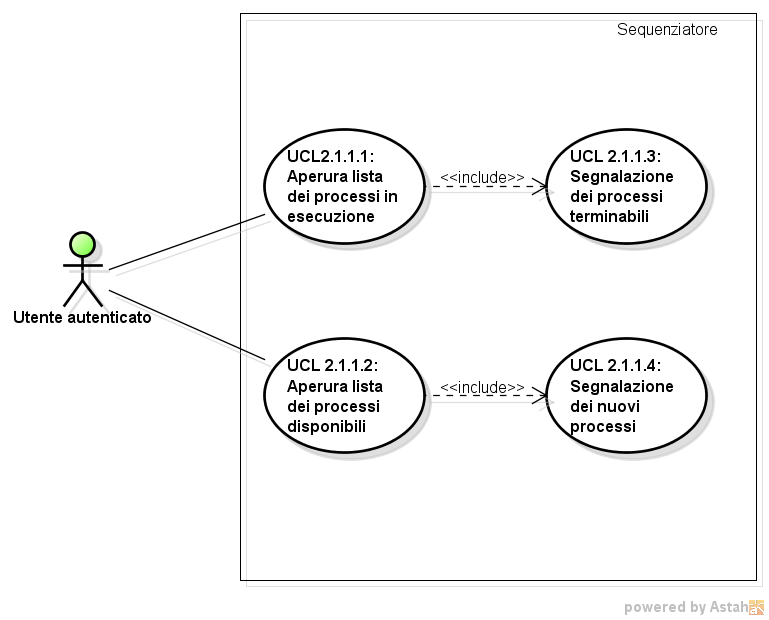
\includegraphics[trim=0cm 0.8cm 0cm 0cm,clip=true,width=%
\textwidth]
{./grafici/L211}
\caption{UCL 2.1.1: Apertura di una lista di processi}
\end{figure}
\begin{itemize}
\item \textbf{Attori:} Utente autenticato;
\item \textbf{Descrizione:} L'utente può scegliere e aprire una lista di processi;
\item \textbf{Precondizione:} L'utente vuole scegliere un processo tra quelli a cui può partecipare;
\item \textbf{Scenario principale:}
\begin{itemize}
\item L'utente può aprire la lista dei processi a cui è iscritto (UCL 2.1.1.1);
\item L'utente può aprire la lista dei processi a cui non è iscritto (UCL 2.1.1.2).
\end{itemize}
%\item \textbf{Scenario alternativo:}
\item \textbf{Inclusioni:}
\begin{itemize}
\item I processi in attesa di terminazione vengono segnalati all'utente;
\item I nuovi processi vengono segnalati all'utente.
\end{itemize}
%\item \textbf{Estensioni:}
\item \textbf{Postcondizione:} Il sistema ha visualizzato la lista dei processi scelta dall'utente.
\end{itemize}

\hypertarget{L2.1.1.1}{}
\bookmark[dest=L2.1.1.1,level=5]{UCL 2.1.1.1: Apertura lista dei processi in esecuzione}
\subsubsection{UCL 2.1.1.1: Apertura lista dei processi in esecuzione}
\begin{itemize}
\item \textbf{Attori:} Utente autenticato;
\item \textbf{Descrizione:} L'utente può aprire e visualizzare la lista dei processi in esecuzione, cioè quelli a cui è già iscritto;
\item \textbf{Precondizione:} L'utente vuole aprire la lista dei processi a cui è iscritto;
\item \textbf{Scenario principale:} L'utente può aprire e visualizzare la lista dei processi in esecuzione, cioè quelli a cui è già iscritto;
%\item \textbf{Scenario alternativo:}
%\item \textbf{Estensioni:}
\item \textbf{Postcondizione:} Il sistema ha visualizzato la lista dei processi a cui l'utente è iscritto.
\end{itemize}

\hypertarget{L2.1.1.2}{}
\bookmark[dest=L2.1.1.2,level=5]{UCL 2.1.1.2: Apertura lista dei processi disponibili}
\subsubsection{UCL 2.1.1.2: Apertura lista dei processi disponibili}
\begin{itemize}
\item \textbf{Attori:} Utente autenticato;
\item \textbf{Descrizione:} L'utente può aprire e visualizzare la lista dei processi disponibili, cioè quelli a cui non è iscritto;
\item \textbf{Precondizione:} L'utente vuole aprire la lista dei processi disponibili;
\item \textbf{Scenario principale:} L'utente può aprire e visualizzare la lista dei processi disponibili, cioè quelli a cui non è iscritto;
%\item \textbf{Scenario alternativo:}
%\item \textbf{Estensioni:}
\item \textbf{Postcondizione:} Il sistema ha visualizzato la lista dei processi a cui l'utente non è iscritto.
\end{itemize}

\hypertarget{L2.1.1.3}{}
\bookmark[dest=L2.1.1.3,level=5]{UCL 2.1.1.3: Segnalazione dei processi terminabili}
\subsubsection{UCL 2.1.1.3: Segnalazione dei processi terminabili}
\begin{itemize}
\item \textbf{Attori:} Utente autenticato;
\item \textbf{Descrizione:} I processi terminati presenti nella lista dei processi in esecuzione, vengono segnalati all'utente;
\item \textbf{Precondizione:} L'utente sta visualizzando la lista dei processi in esecuzione;
\item \textbf{Scenario principale:} I processi terminati presenti nella lista dei processi in esecuzione, vengono segnalati all'utente;
%\item \textbf{Scenario alternativo:}
%\item \textbf{Inclusioni:}
%\item \textbf{Estensioni:}
\item \textbf{Postcondizione:} Il sistema ha evidenziato i processi terminabili dall'utente.
\end{itemize}

\hypertarget{L2.1.1.4}{}
\bookmark[dest=L2.1.1.4,level=5]{UCL 2.1.1.4: Segnalazione dei nuovi processi}
\subsubsection{UCL 2.1.1.4: Segnalazione dei nuovi processi}
\begin{itemize}
\item \textbf{Attori:} Utente autenticato;
\item \textbf{Descrizione:} I processi mai aperti dall'utente, vengono segnalati come nuovi;
\item \textbf{Precondizione:} L'utente sta visualizzando la lista dei processi disponibili;
\item \textbf{Scenario principale:} I processi mai aperti dall'utente, vengono segnalati come nuovi;
%\item \textbf{Scenario alternativo:}
%\item \textbf{Inclusioni:}
%\item \textbf{Estensioni:}
\item \textbf{Postcondizione:} Il sistema ha evidenziato i nuovi processi disponibili all'utente.
\end{itemize}

\hypertarget{L2.1.2}{}
\bookmark[dest=L2.1.2,level=5]{UCL 2.1.2: Filtro dei processi tramite ricerca}
\subsubsection{UCL 2.1.2: Filtro dei processi tramite ricerca}
\begin{itemize}
\item \textbf{Attori:} Utente autenticato;
\item \textbf{Descrizione:} L'utente può filtrare la lista dei processi aperta, effettuano una ricerca testuale;
\item \textbf{Precondizione:} Il sistema ha visualizzato la lista dei processi scelta dall'utente;
\item \textbf{Scenario principale:} L'utente può effettuare una ricerca testuale per ricercare un processo;
%\item \textbf{Inclusioni:}
%\item \textbf{Estensioni:}
\item \textbf{Postcondizione:} Il sistema ha filtrato la lista dei processi che ora è composta dai soli processi che contengono il testo ricercato.
\end{itemize}

\hypertarget{L2.1.3}{}
\bookmark[dest=L2.1.3,level=5]{UCL 2.1.3: Selezione di un processo}
\subsubsection{UCL 2.1.3: Selezione di un processo}
\begin{itemize}
\item \textbf{Attori:} Utente autenticato;
\item \textbf{Descrizione:} L'utente può selezionare un processo dalla lista dei processi precedentemente aperta;
\item \textbf{Precondizione:} L'utente sta visualizzando una lista di uno o più processi;
\item \textbf{Scenario principale:} L'utente può selezionare un processo dalla lista dei processi precedentemente aperta;
%\item \textbf{Scenario alternativo:}
%\item \textbf{Inclusioni:}
%\item \textbf{Estensioni:}
\item \textbf{Postcondizione:} Il sistema è pronto per la gestione del processo scelto.
\end{itemize}

\hypertarget{L2.2}{}
\bookmark[dest=L2.2,level=5]{UCL 2.2: Visualizzazione della descrizione di un processo}
\subsubsection{UCL 2.2: Visualizzazione della descrizione di un processo}
\begin{itemize}
\item \textbf{Attori:} Utente autenticato;
\item \textbf{Descrizione:} Nella pagina di gestione di un processo selezionato l'utente può visualizzarne la descrizione, che spiega lo scopo del processo;
\item \textbf{Precondizione:} Il sistema ha aperto la pagina di gestione di un processo;\\
\item \textbf{Scenario principale:} L'utente può visualizzare la descrizione del processo;
%\item \textbf{Estensioni:} 
%\item \textbf{Inclusioni:} 
%\item \textbf{Scenario alternativo:} 
\item \textbf{Postcondizione:} Il sistema ha visualizzato la descrizione del processo gestito.
\end{itemize}

\hypertarget{L2.3}{}
\bookmark[dest=L2.3,level=5]{UCL 2.3: Iscrizione ad un processo}
\subsubsection{UCL 2.3: Iscrizione ad un processo}
\begin{itemize}
\item \textbf{Attori:} Utente autenticato;
\item \textbf{Descrizione:} L'utente può iscriversi ad un processo a cui non è ancora iscritto;
\item \textbf{Precondizione:} Il sistema ha aperto la pagina di gestione di un processo e l'utente non è iscritto ad esso;
\item \textbf{Scenario principale:} L'utente può iscriversi ad un processo a cui non è ancora iscritto;
%\item \textbf{Scenario alternativo:}
%\item \textbf{Inclusioni:}
%\item \textbf{Estensioni:}
\item \textbf{Postcondizione:} L'utente è iscritto al processo gestito e il sistema è pronto per la sua esecuzione.
\end{itemize}

\hypertarget{L2.4}{}
\bookmark[dest=L2.4,level=5]{UCL 2.4: Esecuzione di un processo}
\subsubsection{UCL 2.4: Esecuzione di un processo}
\begin{figure}[H]
\centering
\includegraphics[trim=0cm 0.8cm 0cm 0cm,clip=true,scale=0.75]%
{./grafici/L24}
\caption{UCL 2.4: Esecuzione di un processo}
\end{figure}
\begin{itemize}
\item \textbf{Attori:} Utente autenticato;
\item \textbf{Descrizione:} L'utente può visualizzare lo stato di avanzamento e i criteri di terminazione del processo e procedere all'esecuzione di un passo;
\item \textbf{Precondizione:} Il sistema ha aperto la pagina di gestione di un processo e l'utente è iscritto ad esso;
\item \textbf{Flusso principale degli eventi:}
\begin{enumerate}
\item L'utente può visualizzazione i criteri di terminazione del processo (UCL 2.4.1);
\item L'utente può visualizzare lo stato dell'esecuzione del processo (UCL 2.4.2);
\item L'utente può visualizzare la lista dei passi in corso (UCL 2.4.3);
\item L'utente può eseguire un passo del processo (UCL 2.4.4);
\item L'utente può concludere l'esecuzione di un processo (UCL 2.4.5).
\end{enumerate} 
%\item \textbf{Inclusioni:}
\item \textbf{Estensioni:} L'utente può saltare un passo facoltativo (UCL 2.4.6).
\item \textbf{Postcondizione:} Il sistema ha eseguito e salvato le operazioni effettuate dall'utente sul processo gestito.
\end{itemize}

\hypertarget{L2.4.1}{}
\bookmark[dest=L2.4.1,level=5]{UCL 2.4.1: Visualizzazione dei criteri di terminazione di un processo}
\subsubsection{UCL 2.4.1: Visualizzazione dei criteri di terminazione di un processo}
\begin{figure}[H]
\centering
\includegraphics[trim=0cm 0.8cm 0cm 0cm,clip=true,scale=0.75]%
{./grafici/L241}
\caption{UCL 2.4.1: Visualizzazione dei criteri di terminazione di un processo}
\end{figure}
\begin{itemize}
\item \textbf{Attori:} Utente autenticato;
\item \textbf{Descrizione:} L'utente può visualizzare i criteri di terminazione del processo selezionato. Questi criteri sono il completamento del processo da parte di un certo numero di utenti ed eventualmente una precisa data di scadenza;
\item \textbf{Precondizione:} Il sistema ha aperto la pagina di gestione di un processo non terminato e l'utente è iscritto ad esso;
\item \textbf{Scenario principale:}
\begin{itemize}
\item L'utente può visualizzare il numero di completamenti che causano la terminazione del processo (UCL 2.4.1.1);
\item L'utente può visualizzare l'eventuale data di scadenza del processo (UCL 2.4.1.2).
\end{itemize}
%\item \textbf{Estensioni:}
%\item \textbf{Inclusioni:}
%\item \textbf{Scenario alternativo:} 
\item \textbf{Postcondizione:} Il sistema ha visualizzato i criteri di terminazione del processo gestito.
\end{itemize}

\hypertarget{L2.4.1.1}{}
\bookmark[dest=L2.4.1.1,level=5]{UCL 2.4.1.1: Visualizzazione massimo numero possibile di completamenti del processo}
\subsubsection{UCL 2.4.1.1: Visualizzazione massimo numero possibile di completamenti del processo}
\begin{itemize}
\item \textbf{Attori:} Utente autenticato;
\item \textbf{Descrizione:} L'utente può visualizzare il numero di completamenti del processo, necessario e sufficiente a causarne la terminazione;
\item \textbf{Precondizione:} Il sistema ha aperto la pagina di gestione di un processo non terminato e l'utente è iscritto ad esso;
\item \textbf{Scenario principale:}  L'utente può visualizzare il numero massimo di completamenti del processo;
%\item \textbf{Estensioni:}
%\item \textbf{Inclusioni:}
%\item \textbf{Scenario alternativo:} 
\item \textbf{Postcondizione:} Il sistema ha visualizzato il numero di completamenti che causano la terminazione del processo.
\end{itemize}

\hypertarget{L2.4.1.2}{}
\bookmark[dest=L2.4.1.2,level=5]{UCL 2.4.1.2: Visualizzazione data di scadenza del processo}
\subsubsection{UCL 2.4.1.2: Visualizzazione data di scadenza del processo}
\begin{itemize}
\item \textbf{Attori:} Utente autenticato;
\item \textbf{Descrizione:} L'utente può visualizzare l'eventuale data di scadenza del processo;
\item \textbf{Precondizione:} Il sistema ha aperto la pagina di gestione di un processo  non terminato e con una data di scadenza, e l'utente è iscritto ad esso;
\item \textbf{Scenario principale:} L'utente può visualizzare l'eventuale data di scadenza del processo;
%\item \textbf{Estensioni:}
%\item \textbf{Inclusioni:}
%\item \textbf{Scenario alternativo:} 
\item \textbf{Postcondizione:} Il sistema ha visualizzato la data di scadenza del processo.
\end{itemize}

\hypertarget{L2.4.2}{}
\bookmark[dest=L2.4.2,level=5]{UCL 2.4.2: Visualizzazione dello stato del processo}
\subsubsection{UCL 2.4.2: Visualizzazione dello stato del processo}
\begin{figure}[H]
\centering
\includegraphics[trim=0cm 0.8cm 0cm 0cm,clip=true,scale=0.75]%
{./grafici/L242}
\caption{UCL 2.4.2: Visualizzazione dello stato del processo}
\end{figure}
\begin{itemize}
\item \textbf{Attori:} Utente autenticato;
\item \textbf{Descrizione:} L'utente può visualizzare informazioni sullo stato di avanzamento del processo. In particolare può visualizzare il numero di passi completati, il totale dei passi, il numero di utenti che hanno completato il processo e il numero di utenti iscritti al processo;
\item \textbf{Precondizione:} Il sistema ha aperto la pagina di gestione di un processo e l'utente è iscritto ad esso;
\item \textbf{Scenario principale:}
\begin{itemize}
\item L'utente visualizza il numero di passi che ha completato (UCL 2.4.2.1);
\item L'utente visualizza il numero totale di passi del processo (UCL 2.4.2.2);
\item L'utente visualizza il numero di utenti che hanno completato il processo (UCL 2.4.2.3);
\item L'utente visualizza il numero di utenti iscritti al processo (UCL 2.4.2.4).
\end{itemize}
%\item \textbf{Estensioni:}
%\item \textbf{Inclusioni:}
%\item \textbf{Scenario alternativo:} 
\item \textbf{Postcondizione:} Il sistema ha visualizzato le informazioni sullo stato di avanzamento del processo.
\end{itemize}

\hypertarget{L2.4.2.1}{}
\bookmark[dest=L2.4.2.1,level=5]{UCL 2.4.2.1: Visualizzazione numero di passi completati}
\subsubsection{UCL 2.4.2.1: Visualizzazione numero di passi completati}
\begin{itemize}
\item \textbf{Attori:} Utente autenticato;
\item \textbf{Descrizione:} L'utente può visualizzare il numero di passi completati del processo;
\item \textbf{Precondizione:} Il sistema ha aperto la pagina di gestione di un processo e l'utente è iscritto ad esso;
\item \textbf{Scenario principale:} L'utente può visualizzare il numero di passi completati del processo;
%\item \textbf{Scenario alternativo:}
%\item \textbf{Inclusioni:}
%\item \textbf{Estensioni:}
\item \textbf{Postcondizione:} Il sistema ha visualizzato il numero di passi del processo gestito completati dall'utente.
\end{itemize}

\hypertarget{L2.4.2.2}{}
\bookmark[dest=L2.4.2.2,level=5]{UCL 2.4.2.2: Visualizzazione numero totale dei passi}
\subsubsection{UCL 2.4.2.2: Visualizzazione numero totale dei passi}
\begin{itemize}
\item \textbf{Attori:} Utente autenticato;
\item \textbf{Descrizione:} L'utente può visualizzare il numero di passi del processo;
\item \textbf{Precondizione:} Il sistema ha aperto la pagina di gestione di un processo e l'utente è iscritto ad esso;
\item \textbf{Scenario principale:} L'utente può visualizzare il numero di passi del processo;
%\item \textbf{Scenario alternativo:}
%\item \textbf{Inclusioni:}
%\item \textbf{Estensioni:}
\item \textbf{Postcondizione:} Il sistema ha visualizzato il numero dei passi del processo gestito.
\end{itemize}

\hypertarget{L2.4.2.3}{}
\bookmark[dest=L2.4.2.3,level=5]{UCL 2.4.2.3: Visualizzazione numero di completamenti del processo}
\subsubsection{UCL 2.4.2.3: Visualizzazione numero di completamenti del processo}
\begin{itemize}
\item \textbf{Attori:} Utente autenticato;
\item \textbf{Descrizione:} L'utente può visualizzare il numero di utenti che hanno completato il processo gestito;
\item \textbf{Precondizione:} Il sistema ha aperto la pagina di gestione di un processo e l'utente è iscritto ad esso;
\item \textbf{Scenario principale:} L'utente può visualizzare il numero di utenti che hanno completato il processo gestito;
%\item \textbf{Scenario alternativo:}
%\item \textbf{Inclusioni:}
%\item \textbf{Estensioni:}
\item \textbf{Postcondizione:} Il sistema ha visualizzato di utenti che hanno completato il processo gestito.
\end{itemize}

\hypertarget{L2.4.2.4}{}
\bookmark[dest=L2.4.2.4,level=5]{UCL 2.4.2.4: Visualizzazione numero di iscritti al processo}
\subsubsection{UCL 2.4.2.4: Visualizzazione numero di iscritti al processo}
\begin{itemize}
\item \textbf{Attori:} Utente autenticato;
\item \textbf{Descrizione:} L'utente può visualizzare il numero di utenti iscritti al processo;
\item \textbf{Precondizione:} Il sistema ha aperto la pagina di gestione di un processo e l'utente è iscritto ad esso;
\item \textbf{Scenario principale:} L'utente può visualizzare il numero di utenti iscritti al processo;
%\item \textbf{Scenario alternativo:}
%\item \textbf{Inclusioni:}
%\item \textbf{Estensioni:}
\item \textbf{Postcondizione:} Il sistema ha visualizzato il numero di utenti iscritti al processo gestito.
\end{itemize}

\hypertarget{L2.4.3}{}
\bookmark[dest=L2.4.3,level=5]{UCL 2.4.3: Visualizzazione della lista dei passi in corso}
\subsubsection{UCL 2.4.3: Visualizzazione della lista dei passi in corso}
\begin{itemize}
\item \textbf{Attori:} Utente autenticato;
\item \textbf{Descrizione:} L'utente può visualizzare la lista passi non ancora conclusi, immediatamente successivi agli ultimi passi superati;
\item \textbf{Precondizione:} Il sistema ha aperto la pagina di gestione di un processo non terminato, l'utente è iscritto ad esso e non lo ha concluso;
\item \textbf{Scenario principale:} L'utente può visualizzare la lista passi non ancora conclusi;
%\item \textbf{Scenario alternativo:}
%\item \textbf{Inclusioni:}
%\item \textbf{Estensioni:}
\item \textbf{Postcondizione:} Il sistema ha visualizzato la lista dei passo in corso ed è pronto per gestirli.
\end{itemize}

\hypertarget{L2.4.4}{}
\bookmark[dest=L2.4.4,level=5]{UCL 2.4.4: Esecuzione di un passo}
\subsubsection{UCL 2.4.4: Esecuzione di un passo}
\begin{figure}[H]
\centering
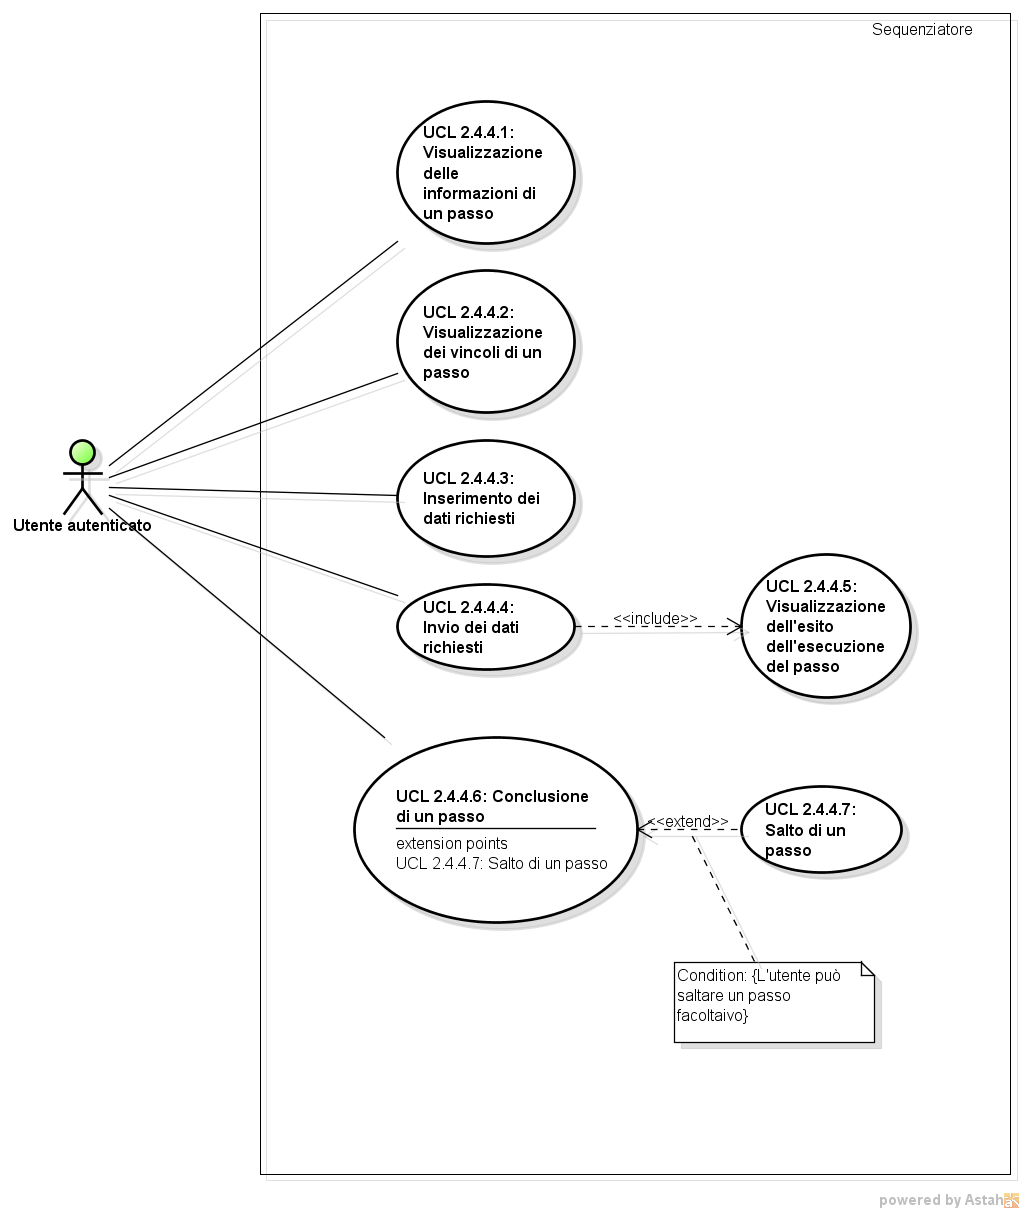
\includegraphics[trim=0cm 0.8cm 0cm 0cm,clip=true,width=%
\textwidth]
{./grafici/L244}
\caption{UCL 2.4.4: Esecuzione di un passo}
\end{figure}
\begin{itemize}
\item \textbf{Attori:} Utente autenticato;
\item \textbf{Descrizione:} L'utente può visualizzare i criteri di terminazione di un passo del processo, inserire i dati richiesti e procedere all'invio dei dati immessi. In seguito all'invio dei dati l'utente riceverà una notifica;
\item \textbf{Precondizione:} L'utente sta visualizzando la lista dei passi in corso e il sistema è pronto alla loro gestione;
\item \textbf{Flusso principale degli eventi:}
\begin{enumerate}
\item L'utente può visualizzare le informazioni sul passo (UCL 2.4.4.1);
\item L'utente può visualizzare i vincoli di un passo (UCL 2.4.4.2);
\item L'utente può inserire i dati richiesti da un passo (UCL 2.4.4.3);
\item L'utente può inviare al sistema i dati richiesti da un passo (UCL 2.4.4.4);
\item L'utente può concludere un passo (UCL 2.4.4.5).
\end{enumerate}
%\item \textbf{Scenario alternativo:}
\item \textbf{Inclusioni:} l'utente dopo aver inviato i dati può visualizzare l'esito dell'esecuzione del passo;
\item \textbf{Estensioni:} L'utente può saltare i passi opzionali;
\item \textbf{Postcondizione:} Il sistema ha eseguito e salvato le operazioni effettuate dall'utente sul passo eseguito e ritorna alla gestione del processo.
\end{itemize}

\hypertarget{L2.4.4.1}{}
\bookmark[dest=L2.4.4.1,level=5]{UCL 2.4.4.1: Visualizzazione delle informazioni di un passo}
\subsubsection{UCL 2.4.4.1: Visualizzazione delle informazioni di un passo}
\begin{itemize}
\item \textbf{Attori:} Utente autenticato;
\item \textbf{Descrizione:} L'utente può visualizzare l'eventuale descrizione del passo e le eventuali descrizioni dei dati richiesti;
\item \textbf{Precondizione:} Il sistema è pronto alla gestione dei passi del processo;
\item \textbf{Scenario principale:} L'utente può visualizzare l'eventuale descrizione del passo e le eventuali descrizioni dei dati richiesti;
%\item \textbf{Scenario alternativo:}
%\item \textbf{Inclusioni:} l'utente dopo aver inviato i dati può visualizzare l'esito dell'esecuzione del passo;
%\item \textbf{Estensioni:} 
\item \textbf{Postcondizione:} Il sistema ha visualizzato le informazioni sul passo.
\end{itemize}

\hypertarget{L2.4.4.2}{}
\bookmark[dest=L2.4.4.2,level=5]{UCL 2.4.4.2: Visualizzazione dei vincoli di un passo}
\subsubsection{UCL 2.4.4.2: Visualizzazione dei vincoli di un passo}
\begin{figure}[H]
\centering
\includegraphics[trim=0cm 0.8cm 0cm 0cm,clip=true,scale=0.75]%
{./grafici/L2442}
\caption{UCL 2.4.4.2: Visualizzazione dei vincoli di un passo}
\end{figure}
\begin{itemize}
\item \textbf{Attori:} Utente autenticato;
\item \textbf{Descrizione:} L'utente può visualizzare i vincoli sui dati richiesti e sull'approvazione del passo;
\item \textbf{Precondizione:} Il sistema è pronto alla gestione dei passi del processo;
\item \textbf{Scenario principale:}
\begin{itemize}
\item L'utente può visualizzare i vincoli sull'approvazione del passo (UCL 2.4.4.2.1);
\item L'utente può visualizzare i vincoli sulle coordinate (UCL 2.4.4.2.2);
\item L'utente può visualizzare i vincoli temporali (UCL 2.4.4.2.3);
\item L'utente può visualizzare i vincoli sui dati numerici (UCL 2.4.4.2.4).
\end{itemize}
%\item \textbf{Scenario alternativo:}
%\item \textbf{Inclusioni:} l'utente dopo aver inviato i dati può visualizzare l'esito dell'esecuzione del passo;
%\item \textbf{Estensioni:} 
\item \textbf{Postcondizione:} Il sistema ha visualizzato i vincoli sui dati da inserire.
\end{itemize}

\hypertarget{L2.4.4.2.1}{}
\bookmark[dest=L2.4.4.2.1,level=5]{UCL 2.4.4.2.1: Visualizzazione dei vincoli sull'approvazione}
\subsubsection{UCL 2.4.4.2.1: Visualizzazione dei vincoli sull'approvazione}
\begin{itemize}
\item \textbf{Attori:} Utente autenticato;
\item \textbf{Descrizione:} L'utente può visualizzare se il passo gestito richiede l'approvazione del \textit{process owner\ped{G}} per essere concluso;
\item \textbf{Precondizione:} Il sistema è pronto alla gestione dei passi del processo;
\item \textbf{Scenario principale:} L'utente può visualizzare i vincoli sull'approvazione del passo gestito;
%\item \textbf{Scenario alternativo:}
%\item \textbf{Inclusioni:} l'utente dopo aver inviato i dati può visualizzare l'esito dell'esecuzione del passo;
%\item \textbf{Estensioni:} 
\item \textbf{Postcondizione:} Il sistema ha visualizzato i vincoli sull'approvazione del passo gestito.
\end{itemize}

\hypertarget{L2.4.4.2.2}{}
\bookmark[dest=L2.4.4.2.2,level=5]{UCL 2.4.4.2.2: Visualizzazione dei vincoli sulle coordinate}
\subsubsection{UCL 2.4.4.2.2: Visualizzazione dei vincoli sulle coordinate}
\begin{itemize}
\item \textbf{Attori:} Utente autenticato;
\item \textbf{Descrizione:} L'utente può visualizzare i vincoli sui dati geografici richiesti. Questi vincoli sono espressi tramite l'indicazione di un luogo preciso e di un'eventuale raggio di tolleranza rispetto al luogo indicato;
\item \textbf{Precondizione:} Il sistema di gestione del passo gestito richiede l'invio delle coordinate geografiche dell'utente;
\item \textbf{Scenario principale:} L'utente può visualizzare i vincoli sui dati geografici richiesti;
%\item \textbf{Scenario alternativo:}
%\item \textbf{Inclusioni:} l'utente dopo aver inviato i dati può visualizzare l'esito dell'esecuzione del passo;
%\item \textbf{Estensioni:} 
\item \textbf{Postcondizione:} Il sistema ha visualizzato i vincoli sulle coordinate richieste dal passo gestito.
\end{itemize}

\hypertarget{L2.4.4.2.3}{}
\bookmark[dest=L2.4.4.2.3,level=5]{UCL 2.4.4.2.3: Visualizzazione dei vincoli temporali}
\subsubsection{UCL 2.4.4.2.3: Visualizzazione dei vincoli temporali}
\begin{itemize}
\item \textbf{Attori:} Utente autenticato;
\item \textbf{Descrizione:} L'utente può visualizzare gli intervalli temporali in cui l'utente può inviare i dati;
\item \textbf{Precondizione:} Il sistema di gestione del passo gestito richiede la data e l'ora dell'invio dei dati;
\item \textbf{Scenario principale:} L'utente può visualizzare gli intervalli temporali in cui l'utente può inviare i dati; 
%\item \textbf{Scenario alternativo:}
%\item \textbf{Inclusioni:} l'utente dopo aver inviato i dati può visualizzare l'esito dell'esecuzione del passo;
%\item \textbf{Estensioni:} 
\item \textbf{Postcondizione:} Il sistema ha visualizzato i vincoli sui tempi di invio dei dati.
\end{itemize}

\hypertarget{L2.4.4.2.4}{}
\bookmark[dest=L2.4.4.2.4,level=5]{UCL 2.4.4.2.4: Visualizzazione dei vincoli sui dati numerici}
\subsubsection{UCL 2.4.4.2.4: Visualizzazione dei vincoli sui dati numerici}
\begin{itemize}
\item \textbf{Attori:} Utente autenticato;
\item \textbf{Descrizione:} L'utente può visualizzare i vincoli sui dati numerici che possono essere il numero di cifre, la possibilità di inserire cifre decimali o meno, e un eventuale limite superiore o inferiore;
\item \textbf{Precondizione:} Il sistema di gestione del passo gestito richiede l'inserimento di un valore numerico;
\item \textbf{Scenario principale:} L'utente può visualizzare i vincoli sui dati numerici
%\item \textbf{Scenario alternativo:}
%\item \textbf{Inclusioni:} l'utente dopo aver inviato i dati può visualizzare l'esito dell'esecuzione del passo;
%\item \textbf{Estensioni:} 
\item \textbf{Postcondizione:} Il sistema ha visualizzato i vincoli sui dati numerici richiesti dal passo gestito.
\end{itemize}

\hypertarget{L2.4.4.3}{}
\bookmark[dest=L2.4.4.3,level=5]{UCL 2.4.4.3: Inserimento dei dati richiesti}
\subsubsection{UCL 2.4.4.3: Inserimento dei dati richiesti}
\begin{figure}[H]
\centering
\includegraphics[trim=0cm 0.8cm 0cm 0cm,clip=true,scale=0.75]%
{./grafici/L2443}
\caption{UCL 2.4.4.3: Inserimento dei dati richiesti}
\end{figure}
\begin{itemize}
\item \textbf{Attori:} Utente autenticato;
\item \textbf{Descrizione:} L'utente può inserire i dati richiesti per l'esecuzione del passo in corso. Può essere richiesto il caricamento di foto, di testo o di dati numerici. Ogni passo per essere completato richiede almeno l'inserimento e l'invio di un dato; 
\item \textbf{Precondizione:} Il sistema di gestione del passo richiede l'inserimento di uno o più dati;
\item \textbf{Scenario principale:}
\begin{itemize}
\item L'utente può inserire un'immagine (UCL 2.4.4.3.1);
\item L'utente può inserire del testo (UCL 2.4.4.3.2);
\item L'utente può inserire dei dati numerici (UCL 2.4.4.3.3).
\end{itemize}
%\item \textbf{Scenario alternativo:}
%\item \textbf{Inclusioni:}
%\item \textbf{Estensioni:}
\item \textbf{Postcondizione:} I dati inseriti dall'utente sono pronti per essere inviati al sistema.
\end{itemize}

\hypertarget{L2.4.4.3.1}{}
\bookmark[dest=L2.4.4.3.1,level=5]{UCL 2.4.4.3.1: Inserimento di un'immagine}
\subsubsection{UCL 2.4.4.3.1: Inserimento di un'immagine}
\begin{figure}[H]
\centering
\includegraphics[trim=0cm 0.8cm 0cm 0cm,clip=true,scale=0.75]%
{./grafici/L24431}
\caption{UCL 2.4.4.3.1: Inserimento di un'immagine}
\end{figure}
\begin{itemize}
\item \textbf{Attori:} Utente autenticato;
\item \textbf{Descrizione:} L'utente può inserire un'immagine scattando una foto o caricandola dai propri file;
\item \textbf{Precondizione:} Il sistema richiede per il superamento del passo corrente l'inserimento di uno o più immagini;
\item \textbf{Scenario principale:}
\begin{itemize}
\item L'utente può inserire un'immagine scattando una foto (UCL 2.4.4.3.1.1);
\item L'utente può inserire un'immagine caricandola dai propri file (UCL 2.4.4.3.1.2).
\end{itemize}
%\item \textbf{Scenario alternativo:}
%\item \textbf{Inclusioni:}
%\item \textbf{Estensioni:}
\item \textbf{Postcondizione:} L'immagine inserita dall'utente è pronta per essere inviata al sistema.
\end{itemize}

\hypertarget{L2.4.4.3.1.1}{}
\bookmark[dest=L2.4.4.3.1.1,level=5]{UCL 2.4.4.3.1.1: Inserimento di una foto scattata}
\subsubsection{UCL 2.4.4.3.1.1: Inserimento di una foto scattata}
\begin{itemize}
\item \textbf{Attori:} Utente autenticato;
\item \textbf{Descrizione:} L'utente può scattare una foto per inserire l'immagine richiesta dal passo in corso;
\item \textbf{Precondizione:} L'utente vuole scattare una foto per inserire l'immagine richiesta dal passo gestito;
\item \textbf{Scenario principale:} L'utente può scattare una foto per inserire l'immagine richiesta dal passo in corso;
%\item \textbf{Scenario alternativo:}
%\item \textbf{Inclusioni:}
%\item \textbf{Estensioni:}
\item \textbf{Postcondizione:} La foto scattata dall'utente è pronta per essere inviata al sistema.
\end{itemize}

\hypertarget{L2.4.4.3.1.2}{}
\bookmark[dest=L2.4.4.3.1.2,level=5]{UCL 2.4.4.3.1.2: Inserimento di un'immagine da file}
\subsubsection{UCL 2.4.4.3.1.2: Inserimento di un'immagine da file}
\begin{itemize}
\item \textbf{Attori:} Utente autenticato;
\item \textbf{Descrizione:} L'utente può caricare un'immagine dai suoi file per soddisfare la richiesta del passo in corso;
\item \textbf{Precondizione:} L'utente vuole inserire l'immagine richiesta dal passo gestito caricandola dai suoi file;
\item \textbf{Scenario principale:} L'utente può caricare un'immagine dai suoi file per soddisfare la richiesta del passo in corso;
%\item \textbf{Scenario alternativo:}
%\item \textbf{Inclusioni:}
%\item \textbf{Estensioni:}
\item \textbf{Postcondizione:} L'immagine scelta dall'utente è pronta per essere inviata al sistema.
\end{itemize}

\hypertarget{L2.4.4.3.2}{}
\bookmark[dest=L2.4.4.3.2,level=5]{UCL 2.4.4.3.2: Inserimento di dati testuali}
\subsubsection{UCL 2.4.4.3.2: Inserimento di dati testuali}
\begin{itemize}
\item \textbf{Attori:} Utente autenticato;
\item \textbf{Descrizione:} L'utente può inserire i dati testuali richiesti dal passo in corso;
\item \textbf{Precondizione:} Il sistema di gestione del passo richiede l'inserimento di dati testuali;
\item \textbf{Scenario principale:} L'utente può inserire i dati testuali richiesti dal passo in corso;
%\item \textbf{Scenario alternativo:}
%\item \textbf{Inclusioni:}
%\item \textbf{Estensioni:}
\item \textbf{Postcondizione:} Il testo inserito dall'utente è pronto per essere inviato al sistema.
\end{itemize}

\hypertarget{L2.4.4.3.3}{}
\bookmark[dest=L2.4.4.3.3,level=5]{UCL 2.4.4.3.3: Inserimento di dati numerici}
\subsubsection{UCL 2.4.4.3.3: Inserimento di dati numerici}
\begin{itemize}
\item \textbf{Attori:} Utente autenticato;
\item \textbf{Descrizione:} L'utente può inserire i dati numerici richiesti dal passo in corso;
\item \textbf{Precondizione:} Il sistema di gestione del passo richiede l'inserimento di dati numerici;
\item \textbf{Scenario principale:} L'utente può inserire i dati numerici richiesti dal passo in corso;
%\item \textbf{Scenario alternativo:}
%\item \textbf{Inclusioni:}
%\item \textbf{Estensioni:}
\item \textbf{Postcondizione:} I dati numerici inseriti dall'utente sono pronti per essere inviati al sistema.
\end{itemize}

\hypertarget{L2.4.4.4}{}
\bookmark[dest=L2.4.4.4,level=5]{UCL 2.4.4.4: Invio dei dati richiesti}
\subsubsection{UCL 2.4.4.4: Invio dei dati richiesti}
\begin{itemize}
\item \textbf{Attori:} Utente autenticato;
\item \textbf{Descrizione:} L'utente può inviare i dati richiesti che possono essere le immagini, il testo e i valori numerici inseriti dall'utente, oppure informazioni sul contesto di invio. In particolare può essere inviata la data, l'ora e la posizione geografica dell'utente al momento dell'invio. Ogni passo per essere completato richiede almeno l'inserimento e l'invio di un dato;
\item \textbf{Precondizione:} L'utente vuole inviare al sistema i dati richiesti dal passo gestito;
\item \textbf{Scenario principale:} L'utente può inviare i dati richiesti dal passo gestito;
%\item \textbf{Scenario alternativo:}
%\item \textbf{Inclusioni:}
%\item \textbf{Estensioni:}
\item \textbf{Postcondizione:} Il sistema ha ricevuto i dati richiesti per l'esecuzione del passo gestito dall'utente.
\end{itemize}

\hypertarget{L2.4.4.5}{}
\bookmark[dest=L2.4.4.5,level=5]{UCL 2.4.4.5: Visualizzazione dell'esito dell'esecuzione del passo}
\subsubsection{UCL 2.4.4.5: Visualizzazione dell'esito dell'esecuzione del passo}
\begin{itemize}
\item \textbf{Attori:} Utente autenticato;
\item \textbf{Descrizione:} L'utente, dopo l'invio dei dati, visualizza l'esito dell'esecuzione del passo. Il sistema notifica all'utente se i dati che ha inviato sono corretti o se non soddisfano i vincoli di superamento del passo.
Eventuali errori sui dati vengono specificati all'utente che potrà correggerli e inviarli nuovamente.
Se inviati dall'utente richiedono approvazione, l'utente viene avvisato tramite una notifica, e dovrà attendere che il \textit{process owner\ped{G}} controlli i dati prima di visualizzare l'esito dell'esecuzione e proseguire con la gestione del processo.
\item \textbf{Precondizione:} Il sistema ha ricevuto i dati richiesti per l'esecuzione del passo gestito dall'utente;
\item \textbf{Scenario principale:} L'utente può visualizzare l'esito dell'esecuzione del passo gestito;
%\item \textbf{Inclusioni:}
%\item \textbf{Estensioni:}
\item \textbf{Postcondizione:} Il sistema ha visualizzato l'esito dell'invio dei dati ed è pronto per continuare la procedura di esecuzione del passo.
\end{itemize}

\hypertarget{L2.4.4.6}{}
\bookmark[dest=L2.4.4.6,level=5]{UCL 2.4.4.6: Conclusione del passo}
\subsubsection{UCL 2.4.4.6: Conclusione del passo}
\begin{itemize}
\item \textbf{Attori:} Utente autenticato;
\item \textbf{Descrizione:} L'utente che ha ricevuto la notifica che i dati inviati soddisfano i requisiti imposti, può concludere l'esecuzione del passo. Il sistema riprenderà la procedura di gestione del processo, aggiornando i dati presenti;
\item \textbf{Precondizione:} Il sistema ha approvato i dati inviati dall'utente o il passo gestito è facoltativo;
\item \textbf{Scenario principale:} L'utente può concludere l'esecuzione del passo;
\item \textbf{Postcondizione:} Il sistema ha concluso l'esecuzione del passo gestito e ha aggiornato i dati sulla gestione del processo in esecuzione.
\end{itemize}


\hypertarget{L2.4.5}{}
\bookmark[dest=L2.4.5,level=5]{UCL 2.4.5: Conclusione di un processo}
\subsubsection{UCL 2.4.5: Conclusione di un processo}
\begin{figure}[H]
\centering
\includegraphics[trim=0cm 0.8cm 0cm 0cm,clip=true,scale=0.75]%
{./grafici/L245}
\caption{UCL 2.4.5: Conclusione di un processo}
\end{figure}
\begin{itemize}
\item \textbf{Attori:} Utente autenticato;
\item \textbf{Descrizione:} L'utente può visualizzare un report dell'esecuzione di un processo terminato o del quale ha eseguito con successo tutti i passi. Può inoltre concludere definitivamente il processo, rimuovendolo quindi dalla lista dei processi in esecuzione;
\item \textbf{Precondizione:} Il sistema ha aperto la pagina di gestione di un processo terminato o del quale l'utente ha eseguito tutti i passi, ma di cui non ha ancora richiesto la conclusione;
\item \textbf{Scenario principale:}
\begin{enumerate}
\item L'utente può visualizzare e salvare un report sull'esecuzione del processo (UCL 2.4.5.1);
\item L'utente può chiudere il processo (UCL 2.4.5.2).
\end{enumerate}
%\item \textbf{Scenario alternativo:}
%\item \textbf{Inclusioni:}
%\item \textbf{Estensioni:}
\item \textbf{Postcondizione:} Il sistema ha eseguito e salvato le operazioni effettuate dall'utente sul processo gestito concluso.
\end{itemize}

\hypertarget{L2.4.5.1}{}
\bookmark[dest=L2.4.5.1,level=5]{UCL 2.4.5.1: Apertura report finale}
\subsubsection{UCL 2.4.5.1: Apertura report finale}
\begin{itemize}
\item \textbf{Attori:} Utente autenticato;
\item \textbf{Descrizione:} L'utente può visualizzare e salvare un report dell'esecuzione di un processo terminato o del quale ha eseguito con successo tutti i passi. Tale report contiene il responso sull'esecuzione del processo e il riepilogo di tutti i dati inviati dall'utente al sistema durante l'esecuzione dei passi;
\item \textbf{Precondizione:} L'utente vuole visualizzare il report di un processo terminato o del quale ha eseguito tutti i passi, ma di cui non ha ancora richiesto la conclusione;
\item \textbf{Scenario principale:} L'utente può aprire un report finale sull'esecuzione del processo;
%\item \textbf{Scenario alternativo:}
%\item \textbf{Inclusioni:}
%\item \textbf{Estensioni:}
\item \textbf{Postcondizione:} Il sistema ha creato un report dell'esecuzione del processo e può riprendere la procedura di conclusione del processo.
\end{itemize}

\hypertarget{L2.4.5.2}{}
\bookmark[dest=L2.4.5.2,level=5]{UCL 2.4.5.2: Chiusura di un processo}
\subsubsection{UCL 2.4.5.2: Chiusura di un processo}
\begin{itemize}
\item \textbf{Attori:} Utente autenticato;
\item \textbf{Descrizione:} L'utente può eliminare dalla lista dei processi gestiti, un processo terminato o del quale ha eseguito con successo tutti i passi;
\item \textbf{Precondizione:} L'utente vuole chiudere un processo terminato o del quale ha eseguito tutti i passi, ma di cui non ha ancora richiesto la conclusione;
\item \textbf{Scenario principale:} L'utente può chiudere il processo gestito;
%\item \textbf{Scenario principale:}
%\item \textbf{Scenario alternativo:}
%\item \textbf{Inclusioni:}
%\item \textbf{Estensioni:}
\item \textbf{Postcondizione:} Il processo non fa più parte dei processi gestiti dall'utente e il sistema ritorna dalla gestione dei processi.
\end{itemize}

\hypertarget{L2.4.6}{}
\bookmark[dest=L2.4.6,level=5]{UCL 2.4.6: Salto di un passo}
\subsubsection{UCL 2.4.6: Salto di un passo}
\begin{itemize}
\item \textbf{Attori:} Utente autenticato;
\item \textbf{Descrizione:} L'utente per concludere un passo facoltativo, può saltarlo;
\item \textbf{Precondizione:} Il sistema sta gestendo un passo facoltativo e l'utente vuole saltarlo;
\item \textbf{Scenario principale:} L'utente può saltare il passo in esecuzione;
%\item \textbf{Scenario alternativo:}
%\item \textbf{Inclusioni:}
%\item \textbf{Estensioni:}
\item \textbf{Postcondizione:} Il sistema ha concluso l'esecuzione del passo gestito e ha aggiornato i dati sulla gestione del processo in esecuzione.
\end{itemize}
\hypertarget{L2.5}{}
\bookmark[dest=L2.5,level=5]{UCL 2.5: Disiscrizione da un processo}
\subsubsection{UCL 2.5: Disiscrizione da un processo}
\begin{itemize}
\item \textbf{Attori:} Utente autenticato;
\item \textbf{Descrizione:} L'utente può disiscriversi da un processo a cui è iscritto;
\item \textbf{Precondizione:} Il sistema ha aperto la pagina di gestione di un processo e l'utente è iscritto ad esso;
\item \textbf{Scenario principale:} L'utente può disiscriversi dal processo gestito;
%\item \textbf{Scenario alternativo:}
%\item \textbf{Inclusioni:}
%\item \textbf{Estensioni:}
\item \textbf{Postcondizione:} L'utente non è più iscritto al processo gestito.
\end{itemize}

\hypertarget{L3}{}
\bookmark[dest=L3,level=4]{UCL 3: Logout}
\subsubsection{UCL 3: Logout}
\begin{itemize}
	\item \textbf{Attori:} Utente autenticato;
	\item \textbf{Descrizione:} L'utente autenticato richiede di terminare la propria sessione e uscire dal sistema diventando nuovamente utente generico;
	\item \textbf{Precondizione:} L'utente autenticato vuole uscire dal sistema;
	\item \textbf{Scenario principale:} L'utente può concludere la propria sessione;
	\item \textbf{Postcondizione:} L'utente autenticato è uscito dal sistema diventando utente generico.
\end{itemize}